\documentclass[conference,a4paper]{IEEEtran}
\usepackage{graphicx}
\usepackage{url}
\usepackage[hidelinks]{hyperref}
\renewcommand{\ttdefault}{cmtt}
\graphicspath{{docs/figures/}}
\hypersetup{pdftitle={Instruction and Data Memory Hierarchy},pdfauthor={Team Architec, Section A}}

\title{Instruction and Data Memory Hierarchy:\\A Simple Harvard and Shared-Memory Comparison}
\author{\IEEEauthorblockN{Suryansh Singh (2401010467), Pranjal Modi (2401010334), Sarvjeet Yadav (2401010424),\\
Abhishek Tripathi (2401010022) and Sameer Khan (2401020054)}
\IEEEauthorblockA{Team Architec, Section A --- MCA Project 9, 2026 --- Newton School of Technology, Rishihood University\\
suryansh.singh2024@nst.rishihood.edu.in}}

\begin{document}
\maketitle
\begin{abstract}
A Harvard controller copies one byte in four cycles. A shared-port
baseline needs six cycles for the same copy. We verify the difference
with six directed simulations and compare both implementations on an
iCE40-HX8K FPGA using post-route static timing analysis.

\end{abstract}

\section{Architecture and Motivation}
Microchip's PIC and AVR cores illustrate how separate instruction
and data buses support prefetch during execution~\cite{pic,avr}.
We isolate that effect by changing the port organization while keeping
the controller, initial images and logical capacity fixed.
Icarus Verilog simulates both configurations together~\cite{icarus}.

\section{Memory System Design}
\subsection{Memories and Controller}
Harvard mode uses a $16\times8$-bit instruction memory and a
$16\times8$-bit data memory. Shared mode uses one $32\times8$-bit
memory with a single address port. Both have 32 bytes in total.
The shared address decoder maps instruction offsets to physical addresses
0--15 and data offsets to addresses 16--31. Fig.~\ref{fig:architecture}
shows both organizations.

The controller contains a four-bit program counter (PC), an eight-bit
instruction register with a valid bit, and an eight-bit accumulator (ACC).
PC advances only when a fetch is accepted. The instruction register holds
the current instruction while PC addresses the next one.

\begin{figure}[t]
\centering
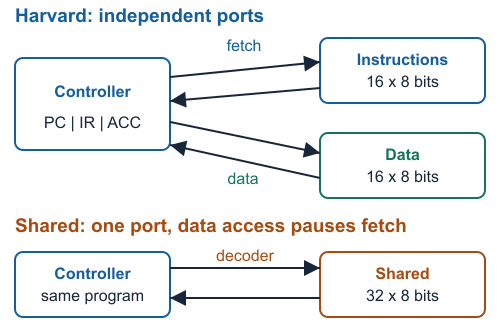
\includegraphics[width=\columnwidth]{architecture_report.png}
\caption{Same controller and capacity, with independent or shared ports.}
\label{fig:architecture}
\end{figure}

\subsection{Instructions and Timing}
The instruction's upper nibble selects the operation and its lower nibble
selects a data address. LOAD (\texttt{1a}) reads data[$a$] into ACC;
STORE (\texttt{2a}) writes ACC to data[$a$]; HALT (\texttt{Fa}) stops.
NOP (\texttt{0a}) performs no data operation. Other opcodes stop with a
fault flag. The low nibble is ignored by NOP and HALT.

Reads are combinational; LOAD captures data and STORE commits its write
at the rising clock edge. A synchronous active-high reset clears the
controller, suppresses memory requests, and retains memory contents.
The simulation uses a 10-ns clock period. Programs must fit in 16 instruction bytes
and end in HALT; the four-bit PC otherwise wraps.

In Harvard mode, fetching the next instruction can overlap the current
LOAD or STORE. In shared mode, data has priority: fetch is blocked, PC
holds, and the instruction-register valid bit clears. The next cycle
fetches the delayed instruction without repeating the previous operation.
HALT suppresses all further memory traffic.

\section{Functional Verification}
The demo image contains \texttt{10 21 F0} (LOAD 0, STORE 1, HALT).
Only data[0] starts at 7. The testbench verifies initialization,
PC advance or hold, exclusive shared-port ownership, operation counts,
all final memory words, and inactivity after HALT. Directed cases in
Table~\ref{tab:results} include an immediate store-to-load dependency,
an illegal instruction, and reset after a committed write.
All six pass using Icarus Verilog 13.0.

\section{Execution Time}
Table~\ref{tab:results} shows measured simulation counts. Counting starts
at the first rising edge after reset release and includes HALT execution.
Reset cycles are excluded.

\begin{table}[t]
\caption{Measured completion cycles for passing scenarios.}
\label{tab:results}
\centering
\begin{tabular}{lrr}
\hline
Scenario & Harvard & Shared \\ \hline
LOAD 0; STORE 1; HALT & 4 & 6 \\
Address boundaries and dependencies & 6 & 10 \\
Two NOPs and HALT & 4 & 4 \\
HALT only & 2 & 2 \\
Invalid opcode & 2 & 2 \\
Restart of longer copy sequence & 8 & 14 \\ \hline
\end{tabular}
\end{table}

\begin{figure}[t]
\centering
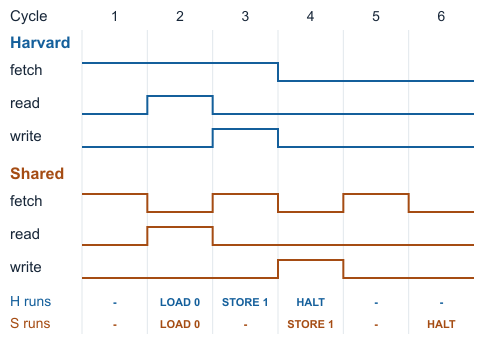
\includegraphics[width=\columnwidth]{waveforms_report.png}
\caption{Demo controls sampled before each rising edge. In cycles 2 and 3,
Harvard fetch overlaps data read and write respectively.}
\label{fig:waveforms}
\end{figure}

Both designs fetch LOAD in cycle 1. Harvard overlaps the read and
write with fetches in cycles 2 and 3 (Fig.~\ref{fig:waveforms}).
The shared machine defers fetch during data accesses in cycles 2
and 4. Both finish with ACC and data[1] equal to 7.

At a common clock frequency, the three-instruction program has a
$6/4=1.50\times$ speedup. Including pipeline fill and HALT, CPI is
$4/3=1.33$ for Harvard and $6/3=2.00$ for shared memory. Two NOPs
followed by HALT finish in four cycles on both designs because the
program never requests the data port.

\section{FPGA Synthesis and Timing}
We mapped the same top-level module, \texttt{memory\_system}, twice for
a Lattice iCE40-HX8K in a CT256 package. Only the \texttt{SHARED\_BUS}
parameter changes. Both builds use the shipped hex images, the same
observable top-level ports, automatic pin placement, placement seed 1
and a 25 MHz clock constraint. Yosys maps the RTL to iCE40 primitives.
Nextpnr packs, places and routes the cells and estimates the internal
register-to-register clock limit from routed delays. External interface
timing and board operation are outside this measurement.

\input{fpga_results.tex}

Harvard uses one embedded RAM for data: Yosys merges the output
register into its read port. The fixed instruction ROM simplifies to
logic. The shared array maps to flip-flops and multiplexers. Packed
cells can combine a LUT and a flip-flop. Both builds meet 25 MHz.
Their area and timing depend on this memory mapping, program image
and placement. Toolchain: Yosys 0.71+post, nextpnr-ice40 0.11.1
(Homebrew revision 2).

\section{Individual Contributions}
The team assigns integration and reporting to Suryansh Singh,
instruction fetch and PC to Pranjal Modi, data memory and control to
Sarvjeet Yadav, shared-port decoding to Abhishek Tripathi, and
testbench and waveform analysis to Sameer Khan.

\section{Conclusion}
Independent ports remove two fetch stalls in the copy program; both
designs tie when there is no data traffic. At the common 25 MHz target,
four and six cycles translate to 160 and 240 ns respectively.
Reproduce the comparison with \texttt{make demo}, \texttt{make test}
and \texttt{make synth}.

\begin{thebibliography}{3}
\bibitem{pic} Microchip Technology, ``8-bit PIC MCU enhanced mid-range
architectural overview,'' \textit{Developer Help}, Jan. 23, 2024.
[Online]. Available:
\url{https://developerhelp.microchip.com/xwiki/bin/view/products/mcu-mpu/8bit-pic/enhanced-family/mrarch/}.
Accessed: Nov. 8, 2026.
\bibitem{avr} Microchip Technology, ``AVR CPU core,'' \textit{Developer
Help}, Nov. 10, 2023. [Online]. Available:
\url{https://developerhelp.microchip.com/xwiki/bin/view/products/mcu-mpu/8-bit-avr/structure/core/}.
Accessed: Nov. 8, 2026.
\bibitem{icarus} S. Williams and contributors, ``Getting started with
Icarus Verilog,'' \textit{Icarus Verilog documentation}. [Online]. Available:
\url{https://steveicarus.github.io/iverilog/usage/getting_started.html}.
Accessed: Nov. 7, 2026.
\end{thebibliography}
\end{document}
